\documentclass[14pt, aspectratio=169]{beamer}

\usepackage[T2A]{fontenc}
\usepackage[utf8]{inputenc}
\usepackage[bulgarian]{babel}
\usepackage[nointegrals]{wasysym}

\usetheme{tues}

\graphicspath{{assets/}}

\definecolor{bibnote}{HTML}{627293}

\title{Въведение}
\subtitle{Операционни системи}
\author{Ангел Пенчев}
\institute{ТУЕС, XI\textsuperscript{А}}
\date{\today}

\begin{document}

\begin{frame}
  \tableofcontents
\end{frame}

\section{Организация}

\begin{frame}{Занятия}
  \begin{itemize}
    \item Два блока седмично; във всеки от тях един учебен час теория и един
      учебен час практика.
    \item За практическите занятия Ви е необходим \emph{компютър}. В случай, че
      за някой конкретен това не е така, ще предупреждавам своевременно.
  \end{itemize}
\end{frame}

\begin{frame}{Конспект - сбита версия}
  \begin{enumerate}
    \setcounter{enumi}{-1}
    \item Въведение в ОС
    \item Програмиране на \texttt{C}
    \item Памет
    \item Процесор
    \item Файлови системи
    \item Мрежи
    \item Сигурност
  \end{enumerate}
\end{frame}

\section{Преговор}

\begin{frame}{Бройни системи}
  \underline{Какво е бройна система?}
  \bigskip

  \begin{tabular}{@{}p{0.6\textwidth}l@{}}
    $14_{(10)} = 1 \cdot 10^1 + 4 \cdot 10^0$
      & $\implies 14_{(10)}$ \\[0.3em]
    $14_{(10)} = 1 \cdot 2^3 + 1 \cdot 2^2 + 1 \cdot 2^1 + 0 \cdot 2^0$
      & $\implies 1110_{(2)}$ \\[0.3em]
    $14_{(10)} = 1 \cdot 3^2 + 1 \cdot 3^1 + 2 \cdot 3^0$
      & $\implies 112_{(3)}$ \\[0.3em]
    $14_{(10)} = 1 \cdot 8^1 + 6 \cdot 8^0$
      & $\implies 16_{(8)}$ \\[0.3em]
    $14_{(10)} = 14 \cdot 16^0$
      & $\implies 14_{(16)} \equiv E_{(16)}$
  \end{tabular}
\end{frame}

\begin{frame}{Бройни системи}
  \[
    14_{\textcolor<5>{teal}{(10)}} =
    \textcolor<3,5>{violet}{1} \cdot 2^{\textcolor<4,5>{orange}{3}} +
    \textcolor<3,5>{violet}{1} \cdot 2^{\textcolor<4,5>{orange}{2}} +
    \textcolor<3,5>{violet}{1} \cdot 2^{\textcolor<4,5>{orange}{1}} +
    \textcolor<3,5>{violet}{0} \cdot 2^{\textcolor<4,5>{orange}{0}} =
    1110_{\textcolor<2,5>{cyan}{(2)}}
  \]
  \bigskip

  \hspace*{1cm}\visible<2,5>{\textcolor{cyan}{База}}\par\smallskip
  \hspace*{1cm}\visible<3,5>{\textcolor{violet}{Коефициенти}}\par\smallskip
  \hspace*{1cm}\visible<4,5>{\textcolor{orange}{Позиции}}\par\smallskip
  \noindent\visible<5>{От значение е и \textcolor{teal}{базата} на
    първоначалната бройна система база.}
\end{frame}

\begin{frame}{Бройни системи}
  \begin{itemize}
    \item Най-важните бройни системи за нас са двоична и шестнайсетична.
    \item Първата, заради нейната тясна връзка с хардуера, върху който се
      изпълняват нашите програми. Ще бележим с префикс \texttt{0b}.
    \item Втората, защото е много лесно преобразуването ѝ към двоична и
      обратно. \emph{Защо?} Ще бележим с префикс \texttt{0x}.
  \end{itemize}
\end{frame}

\begin{frame}{Бройни системи}
  \begin{itemize}
    \item Ключовото наблюдение е, че една шестнайсетична цифра описва точно
      половин байт - т.е. четири бита. Най-голямата шестнайсетична цифра е
      \texttt{f}.
  \end{itemize}
  \[
    \begin{aligned}
      \texttt{f}_{(16)} &= 1111_{(2)} \\
      \texttt{ff}_{(16)} &= 11111111_{(2)}
    \end{aligned}
  \]
\end{frame}

\begin{frame}{Бройни системи}
  \begin{itemize}
    \item Превръщаме от двоична към шестнайсетична, разделяйки поредицата от
      битове (започвайки от най-младшия) на групи от по четири (наричаме ги
      тетрада), и на всяка от получените групи съпоставяме съответната
      шестнайсетична цифра.
    \item Обратната посока. Превръщаме от шестнайсетична към двоична, като на
      всяка цифра съпоставяме група от по четири бита.
  \end{itemize}
\end{frame}

\begin{frame}{Десетични представки}
  Представките в системата SI умножават мерната единица по степен на 10 -
  например $1\,\text{km} = 10^3\,\text{m}$, а $1\,\text{ms} = 10^{-3}\,\text{s}$.
  \medskip

  \noindent
  \begin{columns}[T]
    \begin{column}{0.45\textwidth}
      \centering
      \begin{tabular}{@{}lr@{}}
        \toprule
        \textbf{Представка} & \textbf{Множител} \\
        \midrule
        кило (k) & $10^{3}$ \\
        мега (M) & $10^{6}$ \\
        гига (G) & $10^{9}$ \\
        тера (T) & $10^{12}$ \\
        пета (P) & $10^{15}$ \\
        \bottomrule
      \end{tabular}
    \end{column}
    \begin{column}{0.45\textwidth}
      \centering
      \begin{tabular}{@{}lr@{}}
        \toprule
        \textbf{Представка} & \textbf{Множител} \\
        \midrule
        мили (m) & $10^{-3}$ \\
        микро (\textmu) & $10^{-6}$ \\
        нано (n) & $10^{-9}$ \\
        пико (p) & $10^{-12}$ \\
        фемто (f) & $10^{-15}$ \\
        \bottomrule
      \end{tabular}
    \end{column}
  \end{columns}
\end{frame}

\begin{frame}{Няколко важни константи}
  \emph{Уговорка.} За нас един килобайт е 1024 байта. Аналогично имаме
  \[
    \begin{aligned}
      1\,\text{KB} &= 1024\,\text{B} \\
      1\,\text{MB} &= 1024\,\text{KB} \\
      1\,\text{GB} &= 1024\,\text{MB} \\
      1\,\text{TB} &= 1024\,\text{GB} \\
      1\,\text{PB} &= 1024\,\text{TB}
    \end{aligned}
  \]
\end{frame}

\begin{frame}{Няколко важни константи}
  \textbf{Няма} да се придържаме към системата SI, която определя един
  килобайт като 1000 байта, а 1024 байта нарича кибибайт. Важните константи
  са:
  \[
    \begin{aligned}
      1\,\text{KB} &= 2^{10}\,\text{B} \\
      1\,\text{MB} &= 2^{20}\,\text{B} \\
      1\,\text{GB} &= 2^{30}\,\text{B} \\
      1\,\text{TB} &= 2^{40}\,\text{B} \\
      1\,\text{PB} &= 2^{50}\,\text{B}
    \end{aligned}
  \]
\end{frame}

\begin{frame}{Няколко важни константи}
  Тяхното помнене е доста удобно, когато трябва бързо да превърнете
  произволно число - било то отместване във файл или големина на описвано
  множество от побитова карта, в размер.
\end{frame}

\begin{frame}{Индианци и яйца (Endianness)}
  \begin{itemize}
    \item \emph{Пример.} Нека имаме целочислено число, съставено от четири
      байта (\texttt{uint32\_t}). В паметта то се представя чрез поредица от
      съседни байтове - това е неговият \emph{запис}. Програмистът влага на
      тези байтове \emph{смисъл} на число, представено в двоична бройна
      система.
    \item За реда на байтовете (записа) има два общоприети варианта -
      отдясно-наляво или отляво-надясно; т.е. младшите битове се намират
      съответно или най-вдясно, или най-вляво.
  \end{itemize}
\end{frame}

\begin{frame}{Индианци и яйца (Endianness)}
  \begin{figure}
    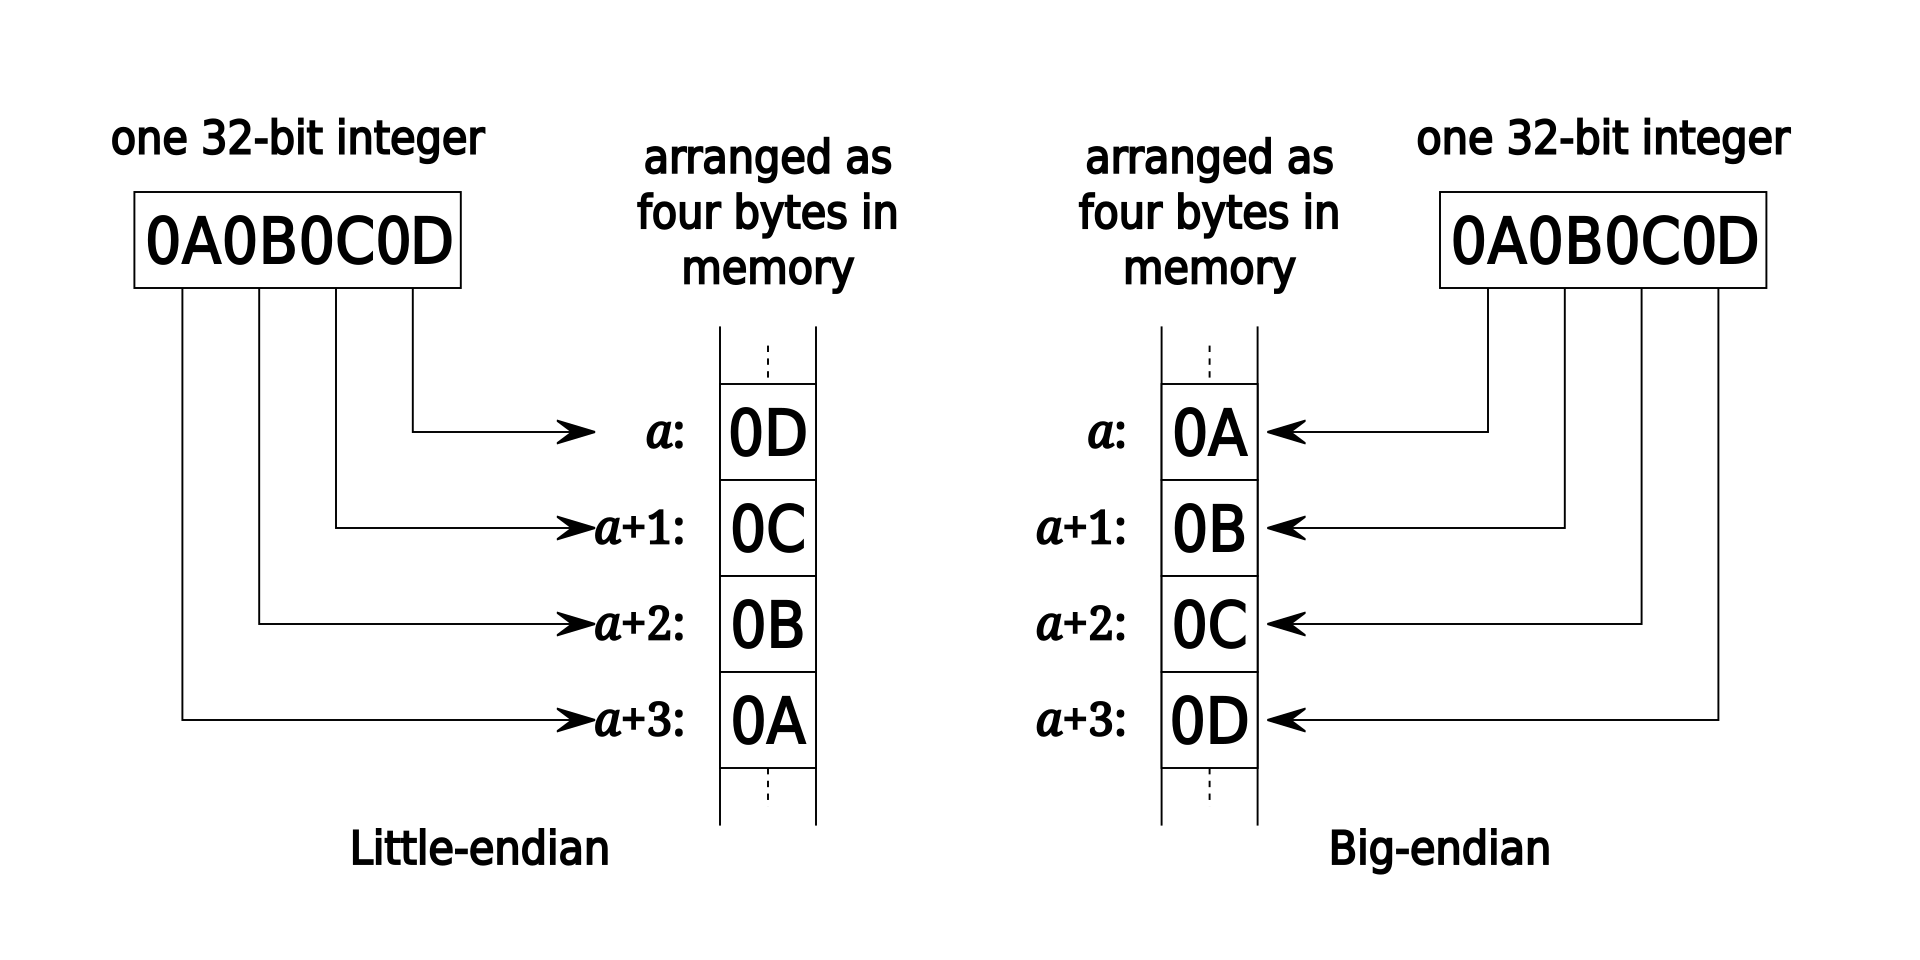
\includegraphics[height=0.55\textheight]{endianness}
    \caption{Илюстрация на endianness при 4-байтово число.}
  \end{figure}
\end{frame}

\begin{frame}{Индианци и яйца (Endianness)}
  \begin{itemize}
    \item Когато байтовете на данните са разположени отдясно-наляво, казваме,
      че се използва big endian. Обратно, ако са отляво-надясно - little
      endian.\footnote{Терминът \emph{endianness} произлиза от творбата
        „Пътешествията на Гъливер“ на Джонатан Суифт, в един епизод от която
        две групи лилипути имат спор за това от кой край трябва да се чупи
        сварено яйце - дали от малкия (little end), или от големия (big end).
        Оттам идват и съответно little-endian и big-endian. Действителна
        връзка с индианци няма. \smiley}
    \item При повечето архитектури (x86, ARM) се използва little-endian.
    \item При комуникация през мрежата се използва big-endian (още наричан
      network order).
  \end{itemize}
\end{frame}

\subsection{Упражнение 1}

\begin{frame}{Упражнение}
  \begin{itemize}
    \item Превърнете 0b111011110011 в шестнайсетична бройна система.
      \answer{0xef3}
    \item Ако горното число беше размер на файл, то колко щеше да бъде голям
      той? \answer{3KB 755B}
    \item Ако горното число беше записът в little-endian, то колко щеше да бъде
      размерът на файла? \answer{0b001111111110 = 0x3fe = 1022B}
    \item 0x8000000, 0x1000, 0x400, 0x10000. \answer{128MB, 4KB, 1KB, 64KB}
    \item Използвайте програма, написана на C, за да проверите дали машината Ви
      използва little- или big-endian за 4-байтово целочислено число.
      \emph{Подсказка.} В \texttt{gdb} използвайте команда \texttt{x/4b \&a},
      където \texttt{a} е вашата променлива.
  \end{itemize}
\end{frame}

\section{Какво е операционна система?}

\begin{frame}{Видове софтуер}
  \emph{Какво е системно програмиране?}
  \bigskip

  \onslide<2>{%
    \renewcommand{\arraystretch}{1.25}%
    \small
    \noindent
    \begin{tabularx}{\textwidth}{@{}XXX@{}}
      \toprule
      \textbf{Компонент} & \textbf{Интерфейс} & \textbf{Функции} \\
      \midrule
      Бизнес модул & Към потребителя - конзола, графично & „Бизнес“ \\
      Библиотеки за общо предназначение & Прост
        & Общи - низове, памет, математика и т.н. \\
      Библиотеки за достъп до хардуер & Логическо устройство
        & Управление на конкретен хардуер \\
      \bottomrule
    \end{tabularx}}
\end{frame}

\begin{frame}{Какво е операционна система?}
  \begin{itemize}
    \item Операционната система (ОС) е софтуер, който споделя и разпределя
      ресурсите на хардуера между различни програми.
    \item Тези програми получават възможност от ОС да не се съобразяват с
      останалите агенти на системата, а само със самата ОС.
    \item Споделянето на ресурсите се осъществява чрез \emph{изолация} и/или
      чрез \emph{заявки}.
    \item \emph{Изолацията} е метод, чрез който ОС показва даден ресурс само и
      единствено на неговия \emph{собственик}.
  \end{itemize}
\end{frame}

\begin{frame}{Какво е операционна система?}
  \begin{itemize}
    \item \emph{Методът на заявките} изисква изрично обръщения на всички
      програми към един и същ ресурс едновременно. Този вид споделяне бива два
      вида - \emph{последователно} (или блокиращо, или синхронно) и
      \emph{паралелно} (или асинхронно). При първото програмата блокира, докато
      не завърши изпратената заявка, докато при второто заявката се поставя в
      опашка за изпълнение и програмата няма контрол в какъв момент точно ще
      бъде изпълнена.
  \end{itemize}
\end{frame}

\begin{frame}{Какво е операционна система?}
  \begin{tabular}{@{}lll@{}}
    \toprule
    \textbf{Ресурс} & \textbf{Абстракция} & \textbf{Метод на споделяне} \\
    \midrule
    Процесор & Нишки & Изолация (и времеделене) \\
    Памет & Адресно пространство & Изолация \\
    Диск & Файлова система & Заявки \\
    Мрежа & Сокети & Заявки \\
    Принтер & Логически принтер & Заявки (асинхронни) \\
    \bottomrule
  \end{tabular}
\end{frame}

\begin{frame}{Какво е операционна система?}
  Изискванията към една ОС още включват -
  \begin{itemize}
    \item Скорост - цената за изпълнение на ОС трябва да бъде минимална.
    \item Надеждност - от издръжливостта на ОС зависят и приложенията.
    \item Изолация между изпълняващите се приложения с цел сигурност.
      Същевременно, начин за споделяне на данни между приложения с цел
      кооперация.
    \item Абстрахиране на конкретния хардуер с цел преносимост.
    \item Удобен интерфейс, за да бъде лесна за употреба.
  \end{itemize}
\end{frame}

\begin{frame}[allowframebreaks]{Структура на ОС}
  След като сме описали задачите, които една ОС трябва да решава, нека опитаме
  да си представим как изглежда горе-долу една такава.

  Нека разгледаме един крайно опростен пример. Имаме приложения, които искат
  да пишат по диска, за да запазват потребителски данни. ОС, в която се
  изпълняват, предоставя интерфейс за работа с диска - приложенията извикват
  \texttt{disk\_write(sector, data)} и ОС се грижи за магията.

  Имаме две непосредствени следствия-проблеми. От една страна това означава,
  че приложение А може да реши да използва сектор 42 и приложение Б да си
  хареса същия сектор. Така те ще бъдат в постоянно състояние на
  \emph{състезание} (на англ. race condition) за данните на сектор 42.

  От втора страна, щом това е просто функция, която може да се извика от
  всеки, то системата е много лесна за компрометиране - произволна програма
  може да изтрие данните на потребителя. Със сигурност нежелан ефект!

  Достигаме до много важен извод - ОС \textbf{не} е просто библиотека с
  функции, които се „грижат за хардуера“. \emph{Откъде точно произлиза
    разликата обаче?}

  \framebreak

  Разликата е, че не всяка програма трябва да може да пише по диска каквото и
  където си пожелае. Това трябва да бъде допустимо при силни ограничения - все
  пак не бива да го забраняваме; дискът наистина е за писане. \emph{Как
    решаваме този проблем?}

  \bigskip
  Понеже разбираме, че трябва дискът да бъде споделен между множество
  програми, си спомняме, че това се случва чрез \emph{заявки} към
  \emph{абстракцията} на диска, а именно - \emph{файловата система}. Така
  решаваме единия проблем.
\end{frame}

\begin{frame}{Структура на ОС}
  Вторият проблем, който представихме, се отнася до сигурността на ОС.
  Решаваме го по следния начин. Въвеждаме понятието \underline{ниво на
    привилегия} (на англ. privilege level или още protection rings). Това е
  свойство на изпълняваща се програма - казваме, че се изпълнява с някакво
  ниво на привилегия.
\end{frame}

\begin{frame}{Структура на ОС}
  \begin{columns}[T]
    \begin{column}{0.48\textwidth}
      \begin{figure}
        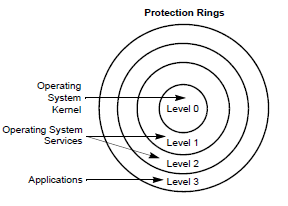
\includegraphics[height=0.5\textheight]{x86-protection-rings}
        \caption{x86 Нива на привилегия}
      \end{figure}
    \end{column}
    \begin{column}{0.48\textwidth}
      \begin{figure}
        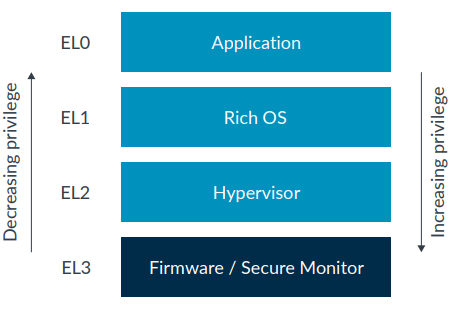
\includegraphics[height=0.5\textheight]{arm-exception-levels}
        \caption{ARM Нива за изключения}
      \end{figure}
    \end{column}
  \end{columns}
\end{frame}

\begin{frame}[allowframebreaks]{Структура на ОС}
  И тогава решението на проблема ни е много просто - за да изпълнява
  \texttt{disk\_write()} (от предходния ни пример), изискваме програмата да се
  изпълнява с ниво на привилегия, което позволява това.

  Както уточнихме вече обаче приложенията не се изпълняват с ниво на
  привилегия, което позволява това. И това е по дизайн.

  Нуждаем се от метод за „промяна на нивото на привилегия“ - изпълняваме си
  приложението, вършейки позволени операции (математически операции, работа с
  низове, взаимодействие с потребител), и в някакъв момент искаме да извикаме
  „забранената“ функция \texttt{disk\_write()}. След като функцията приключи
  работата си, искаме нивото на привилегия да се смени отново - този път към
  началното си състояние.

  Този механизъм се нарича \underline{системно извикване} (на англ. system
  call или накратко syscall). Чрез него потребителско приложение инициира
  работа за ОС. Казваме, че приложението се изпълнява в
  \underline{потребителски режим} (на англ. user mode), а ОС - в
  \underline{режим на ядрото} (на англ. kernel mode). Онази част от ОС, която
  се изпълнява в режим на ядрото, наричаме \underline{ядро} (на англ.
  kernel). При изпълнение в режим на ядрото програмата има достъп до цялата
  системна памет и всички инструкции на процесора, докато при потребителския
  режим ОС се налагат ограничения.

  Нека имаме едно примерно системно извикване \texttt{S()}. Технологията на
  извикване на \texttt{S()} е следната. Когато потребителско приложение А
  желае да изпълни \texttt{S()}, то трябва да задейства \underline{софтуерно
    прекъсване „капан“} (на англ. trap software interrupt), при което
  процесорът ще съхрани състоянието на А, ще премине към режим на ядрото и ще
  премине към изпълнение на обработка на софтуерното прекъсване. При
  обработката на софтуерното прекъсване ще се изпълни работата на
  \texttt{S()}, след което процесорът ще изпълни специална инструкция за
  излизане от капана, ще възвърне състоянието на приложението и то ще
  продължи работата си.

  Забелязваме обаче един важен детайл. При извикването на \texttt{S()} не
  можем просто да посочим неговия адрес. \emph{Защо?}

  Например, ако желаем да отворим файл, за който нямаме права, можем да
  посочим адрес, съответстващ на функцията след проверката за
  правоспособност. Така получаваме способност за отваряне на произволен файл,
  заобикаляйки всякакви проверки за сигурност. Това се нарича
  \underline{уязвимост} (на англ. vulnerability).

  Решението на този проблем е просто. Ядрото използва фиксирана таблица за
  своите системни извиквания. Потребителско приложение уточнява единствено
  индекса на системното извикване, което иска да се изпълни, а ядрото намира
  адреса на съответстващата функция при обработката на софтуерното
  прекъсване.

  Така изяснихме общата постановка на комуникация между ОС и приложенията,
  които ОС управлява.

  Примери за системни извиквания в Linux са \texttt{write}, \texttt{mmap},
  \texttt{shmat} и \texttt{dup}. Общо са около
  \weblink{https://filippo.io/linux-syscall-table/}{500}. Може да се
  запознаете по-обстойно с всеки от тях, използвайки командата \texttt{man 2
    <syscall>}. Можете да разгледате системните извиквания, които Linux
  ядрото предоставя, търсейки макрото \texttt{SYSCALL\_DEFINE}\emph{x}, където
  \emph{x} е цяло число от 0 до 6 (броя параметри) в хранилището на кода -
  \weblink{https://github.com/torvalds/linux.git}{torvalds/linux.git} или в
  индексиращата система
  \weblink{https://elixir.bootlin.com/linux/v6.16/source}{Bootlin}. Да
  отбележим, че когато извикаме например \texttt{write} в своя програма това
  \textbf{не} е системното извикване, както очакваме. Всъщност това е
  функция, дефинирана в стандартната библиотека \texttt{glibc}, която
  извършва описания от нас процес с поставянето на число на определено място
  и предизвикване на софтуерно прекъсване. Такива функции се наричат
  \underline{обвивка} (на англ. wrapper или jacket).

  В MacOS ситуацията е подобна на тази в Linux, поради споделения им
  произход. Можете да разгледате системните извиквания в хранилището на кода
  -
  \weblink{https://github.com/opensource-apple/xnu/blob/master/bsd/kern/syscalls.master}{apple/xnu.git}.
  Там вместо подход с макроси, използват генератор на код.

  В Windows обичайно се използват различни имена на понятията, но
  фундаментално идеята е същата. Наместо системно извикване, популярният
  термин е системна услуга (на англ. system service). Технологията на
  извикване е сходна - числото, подадено от извикващия се използва от
  \emph{диспечера на системни услуги}, за да индексира таблица със самите
  функции, имплементиращи системното извикване. Самите системни извиквания
  са недокументирани официално, но до известна степен следват т.нар. Native
  API, имплементиран в \texttt{NTDLL.dll}, което е „най-ниската точка“,
  изпълняваща се в потребителски режим. Примери за системни услуги в Windows
  са \texttt{NtReadFile} и \texttt{NtWaitForSingleObject}.
\end{frame}

\subsection{Упражнение 2}

\begin{frame}{Упражнение}
  \emph{Забележка:} Понеже все още не сме преминали през темите относно
  \texttt{C}, задачките ще изискват само най-елементарни познания и вярвам, че
  ще се справите \smiley.
  \begin{itemize}
    \item Напишете програма, която приема от стандартния си вход три аргумента
      - име на файл, отместване във файла и низ. Използвайки обвивките на
      системните извиквания за работа с файл - {\rmfamily\textsc{отваряне}},
      {\rmfamily\textsc{писане}} и {\rmfamily\textsc{затваряне}}, програмата
      записва на посоченото отместване данните във файла и приключва.
      \answer{Под Linux и Mac OS използвайте open, write и close, а под
        Windows - CreateFileA, WriteFile и CloseHandle.}
  \end{itemize}
\end{frame}

\begin{frame}{Упражнение}
  \begin{itemize}
    \item Използвайте програма за проследяване на системните извиквания, за да
      разгледате хода на програмата си. В Windows използвайте
      \texttt{Procmon}, в Mac OS - \texttt{sudo dtruss}, а в Linux
      \texttt{strace}. Ако имате други предпочитания, нямам против.
    \item \emph{Забележка (Windows):} Това, което се вижда в колоната
      „Operation“ в \texttt{Procmon} не са системните услуги. Същевременно при
      \emph{\textless десен клик\textgreater} $\rightarrow$ \emph{Stacks} се виждат ясно всички
      извиквания, които се пораждат от функцията, както и това в какъв момент
      точно се преминава към режим на ядрото.
  \end{itemize}
\end{frame}

\begin{frame}
  \begin{figure}
    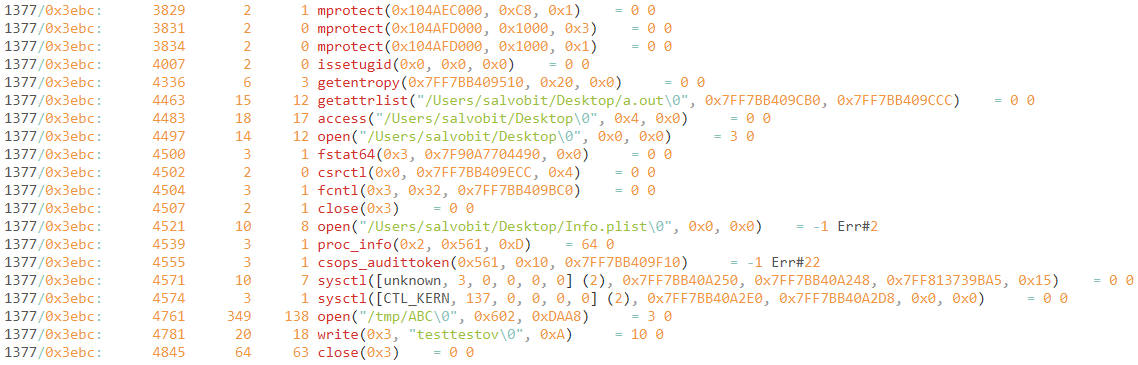
\includegraphics[width=\textwidth]{dtruss}
    \caption{Dtruss (откъс)}
  \end{figure}
\end{frame}

\begin{frame}
  \begin{figure}
    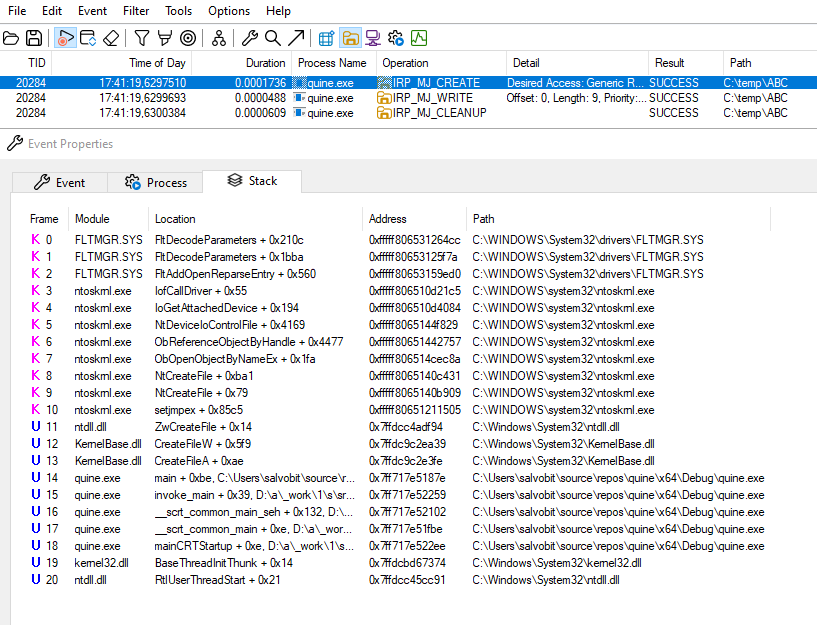
\includegraphics[height=0.72\textheight]{procmon-stack}
    \caption{Procmon (стек)}
  \end{figure}
\end{frame}

\begin{frame}{Обобщение}
  \begin{itemize}
    \item Изложихме основните задачи, които решава една ОС.
    \item Уточнихме какво отличава ОС от библиотека за общо предназначение.
    \item Посочихме двата метода, чрез които ОС споделя ресурсите на машината.
    \item Разгледахме основната техника, използвана от ОС, за да изолират
      изпълнението на приложенията от хардуера.
  \end{itemize}
\end{frame}

\begin{frame}{За четене вкъщи}
  \footnotesize
  \begin{itemize}
    \item \textcolor{tuesnavy}{Remzi H. Arpaci-Dusseau и Andrea C. Arpaci-Dusseau}.
      \emph{Introduction to Operating Systems}.
      {\color{bibnote}\url{https://pages.cs.wisc.edu/~remzi/OSTEP/intro.pdf}.
        Chapter from Operating Systems: Three Easy Pieces, Version 1.10. 2018}
    \item \textcolor{tuesnavy}{Remzi H. Arpaci-Dusseau и Andrea C. Arpaci-Dusseau}.
      \emph{Mechanism: Limited Direct Execution}.
      {\color{bibnote}\url{https://pages.cs.wisc.edu/~remzi/OSTEP/cpu-mechanisms.pdf}.
        Chapter from Operating Systems: Three Easy Pieces, Version 1.10. 2018}
    \item \textcolor{tuesnavy}{David Drysdale}. \emph{Anatomy of a system call, part 1}.
      {\color{bibnote}\url{https://lwn.net/Articles/604287/}. Article from
        LWN.net. 2014}
  \end{itemize}
\end{frame}

\begin{frame}
  \Large Край
\end{frame}

\end{document}
